\begin{frame}
	\myheading{Module 5.5 : Nesterov Accelerated Gradient Descent}
\end{frame}

\begin{frame}
	\begin{overlayarea}{\textwidth}{\textheight}
		\begin{block}{Question}
			\begin{itemize}\justifying
				\item Can we do something  to reduce these oscillations ?
				      \item<2-> Yes, let's look at Nesterov accelerated gradient
			\end{itemize}
		\end{block}
	\end{overlayarea}
\end{frame}

%\subsection{Nesterov accelerated gradient descent}
\begin{frame}
	
	\begin{overlayarea}{\textwidth}{\textheight}
		\vspace{-0.2in}
		\begin{block}{Intuition}
			\begin{itemize}\justifying
				\item<1-> Look before you leap
				\item<2-> Recall that $update_{t} = \gamma\cdot update_{t-1} + \eta \nabla w_{t}$
				\item<3-> So we know that we are going to move by at least by $\gamma\cdot update_{t-1}$ and then a bit more by $\eta \nabla w_{t}$
				\item<4-> Why not calculate the gradient ($\nabla w_{look\_ahead}$) at this partially updated value of $w$ ($w_{look\_ahead} = w_{t} - \gamma\cdot update_{t-1}$)  instead of calculating it using the current value $w_{t}$
			\end{itemize}
		\end{block}
		
		\only<5->{
			\vspace{-0.1in}
			\begin{block}{Update rule for NAG}
				\begin{align*}
					w_{_{look\_ahead}} & = w_{t} - \gamma\cdot update_{t-1}                          \\
					update_t           & = \gamma\cdot update_{t-1} + \eta \nabla w_{_{look\_ahead}} \\
					w_{t+1}            & = w_{t} - update_{t}                                        
				\end{align*}
				We will have similar update rule for $b_t$
			\end{block}
		}
	\end{overlayarea}
\end{frame}

\begin{frame}
	%Mitesh: replace pseudo_code_sgd_crop by code for momentum based sgd
	% replace sgd_error\n.png by mom_error\n.png
	\begin{columns}
		\column{0.5\textwidth}
		\begin{overlayarea}{\textwidth}{\textheight}
			\vspace{-0.15in}
			\begin{figure}
				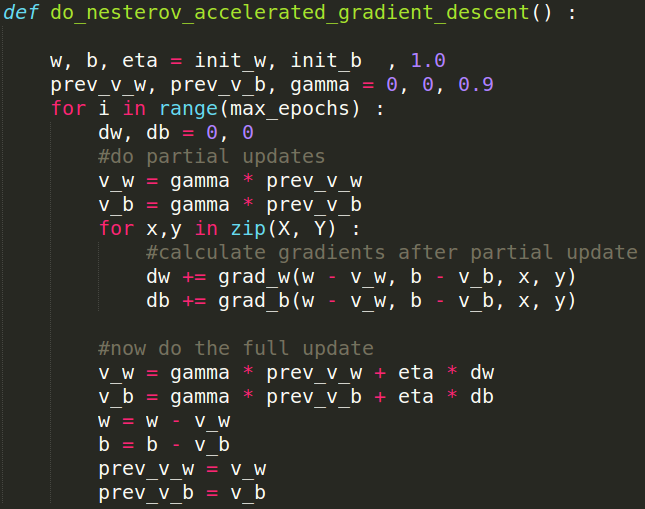
\includegraphics[scale=0.3]{images/module5/pseudo_code_nag_crop.png}
			\end{figure}
		\end{overlayarea}
		
		\column{0.5\textwidth}
		\begin{overlayarea}{\textwidth}{\textheight}
			\vspace{-0.15in}
			\begin{figure}
				\foreach \n in {0,...,40} {%
					\begin{tikzpicture}
						\sbox0{\includegraphics[scale=0.4]{images/module5/nag2/2d_path\n.png}}% get width and height
						\only<\n>{\node[above right,inner sep=0pt] at (0,0)  {\usebox{0}}};
						\only<\n>{\node[red](w) at (0.5\wd0,0.23\ht0) {w}};
						\only<\n>{\node[red](b) at (0,0.67\ht0) {b}};
						\only<\n>{\draw[->, line width=0.2mm](w)--(0.6\wd0,0.23\ht0)};
						\only<\n>{\draw[->, line width=0.2mm](b)--(0,0.8\ht0)};
					\end{tikzpicture}
				}
			\end{figure}
		\end{overlayarea}
	\end{columns}
\end{frame}

\begin{frame}
\end{frame}

\begin{frame}
	\begin{overlayarea}{\textwidth}{\textheight}
		\begin{block}{Observations about NAG}
			\begin{itemize}\justifying
				\item<1-> Looking ahead helps NAG in correcting its course quicker than momentum based gradient descent
				\item<2-> Hence the oscillations are smaller and the chances of escaping the minima valley also smaller
			\end{itemize}
		\end{block}
	\end{overlayarea}
\end{frame}
